
\documentclass{article}
\usepackage[spanish]{babel} %Definir idioma español
\usepackage[utf8]{inputenc} %Codificacion utf-8
\usepackage{amssymb, amsmath, amsbsy, wasysym}
\usepackage{multirow} % para tablas
\usepackage{graphicx}
\title{Actividad 1\\Algoritmos paralelos}
\author{Emmanuel Peto Gutiérrez}
\begin{document}
\maketitle

Ejecuciones del programa:

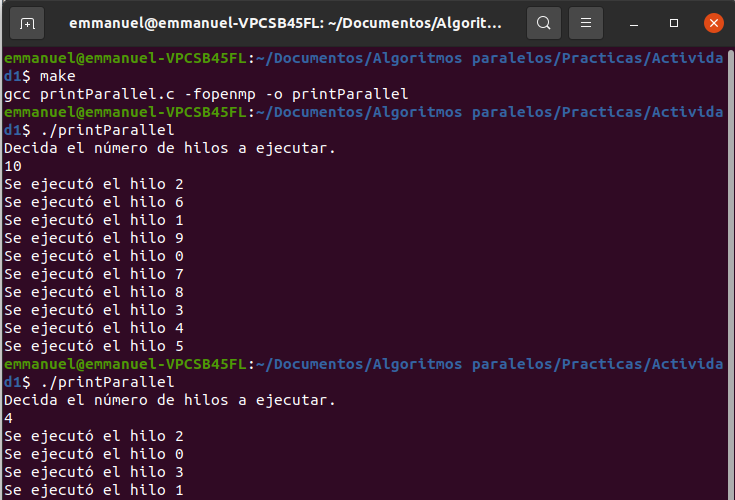
\includegraphics[width=\linewidth]{1}

Datos del equipo:

\begin{center}
\begin{tabular}{|l|l|}
\hline
Marca de equipo & Vaio \\ \hline
Sistema operativo & Ubuntu 20.04.2 LTS \\ \hline
Procesador & Intel Core i5-2450M \\ \hline
Generación & 2 \\ \hline
Núcleos & 2 \\ \hline
\end{tabular}
\end{center}

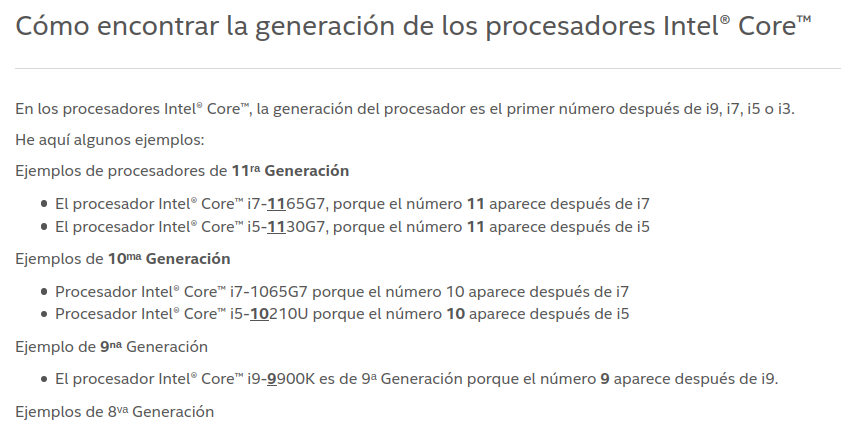
\includegraphics[width=\linewidth]{2}

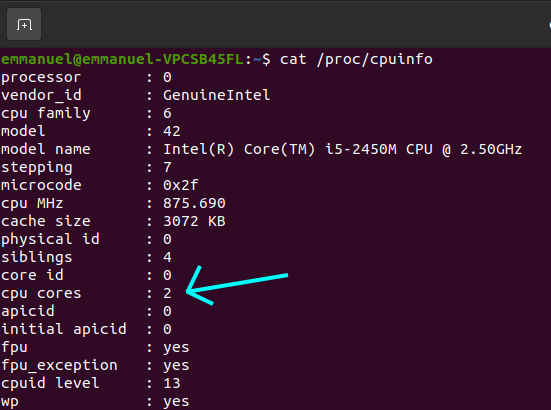
\includegraphics[width=\linewidth]{3}

\end{document}

